\documentclass[14pt,aspectratio=169,xcolor=dvipsnames]{beamer}
\usetheme{SimplePlus}
\usepackage{booktabs}
\usepackage{minted}

\title[short title]{Clase 9: I/O (Input/Output)}
\subtitle{}
\author[NA Barnafi] {Nicolás Alejandro Barnafi Wittwer}
\institute[UC|CMM] 
{
    Pontificia Universidad Católica de Chile \\
    Centro de Modelamiento Matemático
}

\titlegraphic{
    \vspace{-1.8cm}
    \begin{flushright}
      
\includegraphics[height=2.5cm]{../images/logos/puc.png} 
    \end{flushright}
}

\date{04/09/2024}
%\setbeamercovered{transparent}

\begin{document}
%%%%%%%%%%%%%%%%%%%%%%%%%%%%%%%%%%%%%%%%%%%%%%%%%%%%%%%
\begin{frame}
    \maketitle
\end{frame}
%%%%%%%%%%%%%%%%%%%%%%%%%%%%%%%%%%%%%%%%%%%%%%%%%%%%%%%
\begin{frame}\frametitle{Motivación}
    \begin{itemize}
        \item El genoma human pesa $\approx$ 1Gb (película en def standard)
        \item El genoma del krill pesa $\approx$ 12Gb
        \item CPU procesa hasta 64 Kb a la vez
    \end{itemize}
    \hspace{2cm}
\includegraphics[height=4cm]{../images/vitruvio.jpg}
    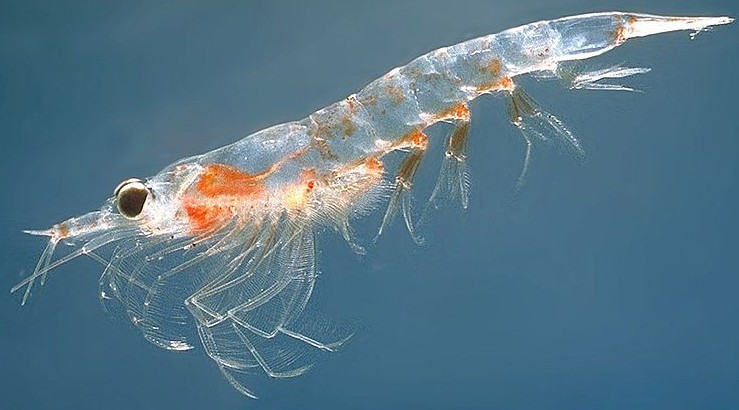
\includegraphics[height=4cm]{../images/krill.jpg}

\pause Necesitamos procesar datos sin cargar todo en memoria (\emph{streams})
\end{frame}
%%%%%%%%%%%%%%%%%%%%%%%%%%%%%%%%%%%%%%%%%%%%%%%%%%%%%%%
\begin{frame}[fragile]\frametitle{Lectura de archivos}
Archivo \texttt{pangrams.txt}:
    \begin{verbatim}
The quick brown fox jumps over the lazy dog
Extraño pan de col y kiwi se quemó bajo fugaz vaho
Ma la volpe col suo balzo ha raggiunto il quieto Fido
Törkylempijä vongahdus
    \end{verbatim}

    \begin{minted}{python}
    f = open("../archivos/pangrams.txt", "r") # (r)ead
    f.read() # o readline(), o readlines()
    f.close()
    \end{minted}
\end{frame}
%%%%%%%%%%%%%%%%%%%%%%%%%%%%%%%%%%%%%%%%%%%%%%%%%%%%%%%
\begin{frame}[fragile]\frametitle{Escritura}
    \begin{minted}{python}
    f = open("../archivos/pangrams.txt", "w") # (w)rite
    f.write() # o writelines()
    f.close()
    \end{minted}

*Es siempre importante \emph{cerrar} el archivo
\end{frame}
%%%%%%%%%%%%%%%%%%%%%%%%%%%%%%%%%%%%%%%%%%%%%%%%%%%%%%%
\begin{frame}[fragile]\frametitle{Uso común}
    Se usa contexto con {\color{purple}\texttt{with}} para cierre automático
    \begin{minted}{python}
    with  open("ejemplo.txt", "w") as f
        f.write("texto nuevo\n") 
    # with
    [...]
    \end{minted}
\end{frame}
%%%%%%%%%%%%%%%%%%%%%%%%%%%%%%%%%%%%%%%%%%%%%%%%%%%%%%%
\begin{frame}[fragile]\frametitle{Modos de lectura}
    \begin{itemize}
        \item 'r': Lee archivo, error si no existe
        \item 'w': Escribe en un archivo. Sobreescribe si existe
        \item 'x': Crea archivo, error si ya existe
        \item 'a': Agrega a archivo al final. Lo crea si no existe.

    \end{itemize}
    
    \vspace{1cm}
    \begin{minted}{python}
    modo = "w" # r|w|x|a
    with open("ejemplo.txt", modo) as f
        [...]
    \end{minted}
\end{frame}
%%%%%%%%%%%%%%%%%%%%%%%%%%%%%%%%%%%%%%%%%%%%%%%%%%%%%%%
\begin{frame}

\idea{Consola...}

\end{frame}
%%%%%%%%%%%%%%%%%%%%%%%%%%%%%%%%%%%%%%%%%%%%%%%%%%%%%%%
\begin{frame}\frametitle{Recap}
    \begin{itemize}
        \item Lectura a través de \emph{stream}
        \item Lectura de archivos con \code{open}
        \item Contexto con \code{with}
        \item Modos de lectura: \code{r},\code{w},\code{a}
    \end{itemize}
\end{frame}
%%%%%%%%%%%%%%%%%%%%%%%%%%%%%%%%%%%%%%%%%%%%%%%%%%%%%%%
\begin{frame}
    \maketitle
\end{frame}
\end{document}
